\documentclass[final,t]{beamer}
\usepackage[size=a0,scale=1.22,orientation=portrait]{beamerposter}
\usepackage[utf8]{inputenc}
\usepackage[T1]{fontenc}
\usepackage{lmodern}
\usepackage{graphicx}
\usepackage{booktabs}
\usepackage{array}
\usepackage{xcolor}
\usepackage{tikz}
\usepackage{fontawesome5}
\usepackage{adjustbox}

\graphicspath{{figures/}}

% --- palette ---
\definecolor{ntured}{HTML}{9F1D35}
\definecolor{accent}{HTML}{1F3A68}
\definecolor{ink}{HTML}{1A1A1A}
\definecolor{soft}{HTML}{4A4A4A}
\definecolor{bg}{HTML}{FBFAF7}

\setbeamercolor{background canvas}{bg=bg}
\setbeamercolor{normal text}{fg=ink}
\setbeamercolor{block title}{fg=white,bg=ntured}
\setbeamercolor{block body}{fg=ink,bg=white}
\setbeamerfont{block title}{size=\Large,series=\bfseries}
\setbeamerfont{block body}{size=\normalsize}
\linespread{1.15}
\setbeamertemplate{navigation symbols}{}
\setbeamertemplate{itemize item}{\color{ntured}\textbf{\textbullet}}
\setbeamertemplate{itemize subitem}{\color{soft}\textbf{--}}

\setbeamertemplate{block begin}{
  \setbeamercolor{block title}{fg=white,bg=ntured}
  \begin{beamercolorbox}[wd=\textwidth,ht=3.2ex,dp=1.6ex,leftskip=0.7cm,colsep*=.0ex]{block title}%
    \usebeamerfont*{block title}\insertblocktitle\strut
  \end{beamercolorbox}
  \nointerlineskip
  \begin{beamercolorbox}[leftskip=0.6cm,rightskip=0.6cm,vmode]{block body}%
  \vspace{0.6cm}
}
\setbeamertemplate{block end}{
  \vspace{0.6ex}\end{beamercolorbox}\vfill
}

\newlength{\colw}
\setlength{\colw}{0.302\paperwidth}
\newlength{\gutter}
\setlength{\gutter}{0.018\paperwidth}
\newlength{\sidemargin}
\setlength{\sidemargin}{0.022\paperwidth}
\newlength{\fullw}
\setlength{\fullw}{0.942\paperwidth}

\begin{document}
\begin{frame}[t]

% ============ TITLE BAR (absolute positioned via tikz) ============
\begin{tikzpicture}[remember picture, overlay]
  \fill[ntured] (current page.north west) rectangle ([yshift=-14.0cm]current page.north east);
  % NTU seal top-left with matching white circular backdrop
  \node[anchor=north west, inner sep=0pt]
    at ([xshift=2.5cm, yshift=-1.0cm]current page.north west) {%
      \begin{tikzpicture}
        \fill[white] (5.5cm,-5.5cm) circle (5.8cm);
        \node[anchor=north west, inner sep=0pt] at (0,0) {
\includegraphics[width=11.0cm]{figures/logos/ntu.png}};
      \end{tikzpicture}%
    };
  % CMU seal top-right with white circular backdrop
  \node[anchor=north east, inner sep=0pt]
    at ([xshift=-2.5cm, yshift=-1.0cm]current page.north east) {%
      \begin{tikzpicture}
        \fill[white] (-5.5cm,-5.5cm) circle (5.8cm);
        \node[anchor=north east, inner sep=0pt] at (0,0) {
\includegraphics[width=11.0cm]{figures/logos/cmu.png}};
      \end{tikzpicture}%
    };
  % Title text centered, narrowed so it does not crowd the two larger seals
  \node[anchor=north, text width=0.58\paperwidth, align=center, inner sep=0pt]
    at ([yshift=-2.2cm]current page.north) {%
      {\color{white}\fontsize{72pt}{84pt}\selectfont\textbf{Probing Functional Correctness in}}\\[0.45cm]
      {\color{white}\fontsize{72pt}{84pt}\selectfont\textbf{Diffusion Language Models}}\\[1.2cm]
      {\color{white}\fontsize{34pt}{40pt}\selectfont\textbf{%
        \makebox[12cm][r]{Guan-Ming Chiu$^{\,1}$,}\hspace{0.5cm}\makebox[12cm][l]{Jeng-Yue Liu$^{\,2}$}%
      }}\\[0.10cm]
      {\color{white!90}\fontsize{24pt}{30pt}\selectfont\textbf{%
        \makebox[12cm][r]{$^{1}$National Taiwan University,}\hspace{0.5cm}\makebox[12cm][l]{$^{2}$Carnegie Mellon University}%
      }}\\[0.08cm]
      {\color{white!90}\fontsize{26pt}{32pt}\selectfont\textbf{%
        \raisebox{-0.18ex}{\faGithub}\hspace{0.45cm}{\fontsize{28pt}{32pt}\selectfont\texttt{github.com/guan404ming/dllm-probing}}%
      }}%
    };
\end{tikzpicture}
\vspace{12.8cm}

% ============ ROW 1: 3 OVERVIEW COLUMNS ============
\begin{columns}[T]
\hspace{\sidemargin}
\begin{column}{\colw}
\begin{block}{Motivation}
\textbf{Diffusion language models} like LLaDA and Dream generate text by \emph{iterative denoising} of all tokens in parallel, not left-to-right. AR probing literature is mature; DLM internals are unexplored, and bidirectional multi-step denoising creates a \emph{fundamentally different} representational landscape.\\
\textbf{Question.} \emph{When} during denoising, and \emph{where} in the layer stack, do hidden states encode whether the output will be functionally correct?\\
\textbf{Why it matters.} The same probe yields a practical lever, \emph{selective generation}, that skips denoising on instances predicted to fail -- saving \textbf{36--98\%} of wasted compute and beating softmax heuristics by 5--20 pts.
\end{block}
\end{column}
\hspace{\gutter}
\begin{column}{\colw}
\begin{block}{Method \& Setup}
\emph{Models.} LLaDA-8B-Instruct (33 layers, block-masked) and Dream-7B-Instruct (29 layers, global-linear).
\vspace{0.25cm}\\
\emph{Tasks} (structural $\to$ reasoning): JSON Schema (272), GSM8K (1{,}319), MBPP (257), ARC-Challenge (1{,}172).
\vspace{0.25cm}\\
\emph{Probing pipeline} on a frozen DLM:
\begin{itemize}\setlength\itemsep{0.9ex}
  \item Run 128-step denoising; extract hidden states at 7 checkpoints $t\in\{0,1,4,16,32,64,127\}$.
  \item Partition generation region into 4 regions, mean-pool $\to$ feature $(L,4,d)$ per step.
  \item Per $(\text{step},\text{layer},\text{region})$: PCA(64) $\to$ \emph{logistic regression}; AUC under 5-fold stratified CV.
\end{itemize}
\end{block}
\end{column}
\hspace{\gutter}
\begin{column}{\colw}
\begin{block}{Key Findings}
\begin{enumerate}\setlength\itemsep{0.9ex}
  \item DLMs \textbf{uniquely accumulate} correctness signal during denoising ($\Delta$AUC $0.08\text{--}0.11$ on reasoning) -- a capacity \emph{absent} in single-pass AR decoding.
  \item Step-0 already carries strong above-chance signal (AUC $0.61\text{--}0.80$), largely reflecting \textbf{prompt difficulty}, not diffusion-specific computation.
  \item Emergence is \textbf{task-dependent}: structural tasks flat from step 0 (AUC $\approx 0.80$); reasoning tasks build gradually across denoising.
  \item \textbf{Divergent layer dynamics}: LLaDA concentrates in upper layers (L22--28); Dream \emph{migrates downward} on simple tasks (L17$\to$L4), tracking pretraining origin.
\end{enumerate}
\end{block}
\end{column}
\hspace{\sidemargin}
\end{columns}

\vfill

% ============ ROW 2: FULL-WIDTH HEATMAP ============
\begin{columns}[T]
\hspace{\sidemargin}
\begin{column}{\fullw}
\begin{block}{AUC heatmaps: layer $\times$ denoising step}
\vspace{0.4cm}
\centering
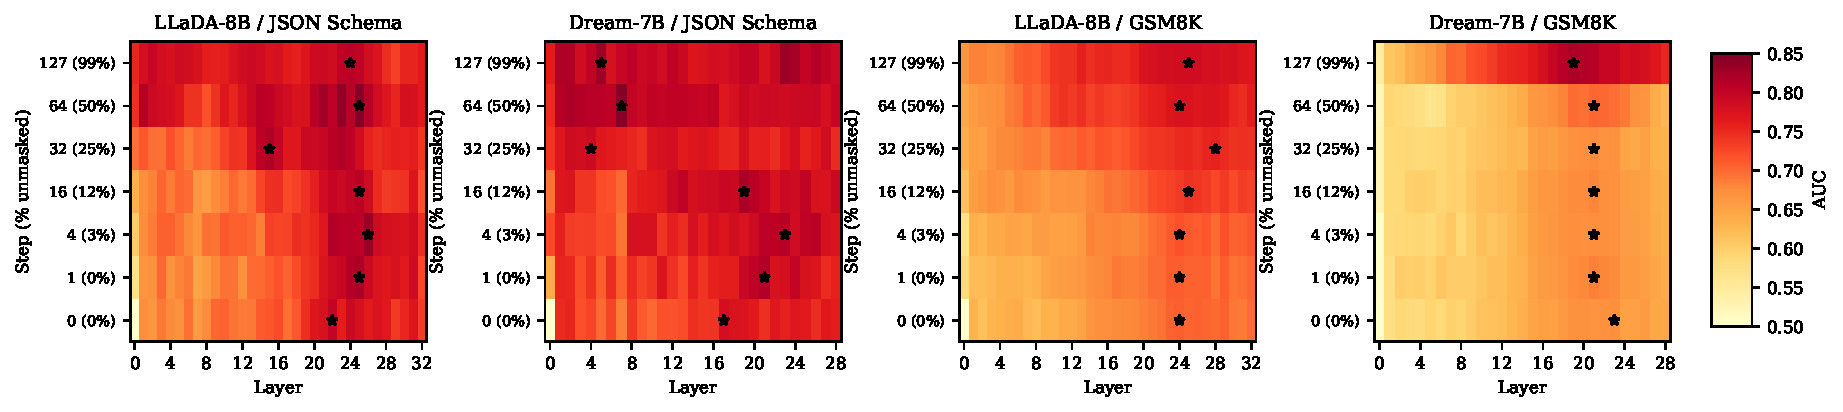
\includegraphics[width=0.99\linewidth]{fig1_heatmap.pdf}\\[0.25cm]
\begin{flushleft}\normalsize Stars mark the best layer per step. \emph{JSON Schema}: signal already strong at step 0, profile flat $\Rightarrow$ \emph{prompt encoding alone} predicts structural correctness. \emph{GSM8K}: gradual emergence as denoising unfolds. Note Dream's \emph{downward layer migration} on JSON Schema -- absent on reasoning tasks.\end{flushleft}
\end{block}
\end{column}
\hspace{\sidemargin}
\end{columns}

\vfill

% ============ ROW 3: AUC CURVES + SELECTIVE GENERATION ============
\begin{columns}[T]
\hspace{\sidemargin}
\begin{column}{0.590\paperwidth}
\begin{block}{Best AUC across layers at each step}
\vspace{0.4cm}
\centering
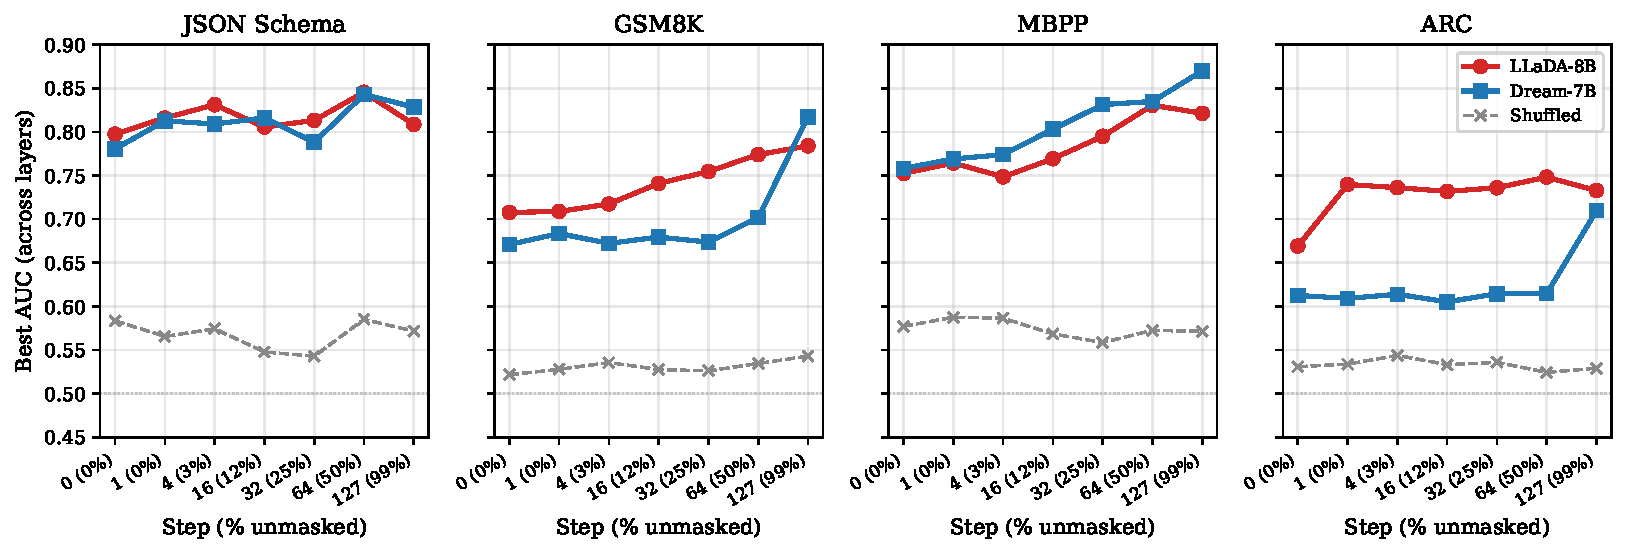
\includegraphics[width=0.99\linewidth]{fig2_auc_curve.pdf}\\[0.20cm]
\begin{flushleft}\normalsize Dashed grey is a shuffled-label control (peaks $\le 0.58$). The four tasks form a clean \emph{structural$\to$reasoning} ladder: JSON is flat ($\approx 0.80$ from step 0); GSM8K, MBPP, ARC climb $0.08\text{--}0.11$ AUC across denoising. LLaDA (red) leads on most tasks; Dream (blue) catches up at full denoising.\end{flushleft}
\end{block}
\end{column}
\hspace{\gutter}
\begin{column}{0.338\paperwidth}
\begin{block}{Selective Generation ($\tau{=}0.80$)}
\vspace{0.8cm}
\centering
\renewcommand{\arraystretch}{1.0}
\setlength{\tabcolsep}{14pt}
\begin{tabular}{l c c c c}
\toprule
 & \textbf{JSON} & \textbf{GSM8K} & \textbf{MBPP} & \textbf{ARC} \\
\midrule
\multicolumn{5}{l}{\textit{LLaDA-8B}}\\
Compute saved & \textbf{98.4} & 61.3 & \textbf{95.5} & \textbf{82.9} \\
Clf. accuracy & 73.5 & 73.5 & 66.5 & 79.6 \\
Majority acc. & 51.5 & 66.3 & 59.1 & 78.2 \\
\midrule
\multicolumn{5}{l}{\textit{Dream-7B}}\\
Compute saved & \textbf{96.7} & 36.0 & \textbf{97.8} & 61.4 \\
Clf. accuracy & 72.4 & 73.5 & 70.0 & 75.9 \\
Majority acc. & 54.0 & 61.5 & 55.6 & 74.5 \\
\bottomrule
\end{tabular}\\[3.3cm]
\begin{flushleft}\small \textbf{Sv}: \% of denoising steps skipped when probe predicts failure. \textbf{Ac}: classification accuracy of probe-as-gate. JSON/MBPP: skip $>95\%$ of compute while clearing the majority baseline by $7\text{--}22$ pts. All values in \%.\end{flushleft}
\end{block}
\end{column}
\hspace{\sidemargin}
\end{columns}

\vfill

% ============ ROW 4: CONTROLS / CONCLUSION / LIMITATIONS ============
\begin{columns}[T]
\hspace{\sidemargin}
\begin{column}{\colw}
\begin{block}{Controls}
\begin{itemize}\setlength\itemsep{0.9ex}
  \item \emph{Shuffled labels}: AUC $\le 0.58$ everywhere; \emph{prompt-length-matched}: avg.\ drop $\le 0.02$.
  \item \emph{Length-matched probe}: AUC drops only $0.00\text{--}0.09$ after matching output length; MBPP shows \emph{no} drop.
  \item \emph{AR baseline} on Qwen-2.5-7B last-prompt token matches DLM step-0 on most tasks, confirming the step-0 signal reflects \textbf{prompt difficulty}, not diffusion-specific computation.
\end{itemize}
\end{block}
\end{column}
\hspace{\gutter}
\begin{column}{\colw}
\begin{block}{Conclusion}
\begin{itemize}\setlength\itemsep{0.9ex}
  \item \emph{First probing study} of DLM hidden states for functional correctness across the full $(\text{layer}, \text{step}, \text{region})$ grid for 2 models $\times$ 4 tasks.
  \item Iterative denoising provides DLMs with $\Delta$AUC $0.08\text{--}0.11$ on reasoning that single-pass AR decoding cannot reach.
  \item Probe confidence enables \emph{offline selective generation} that saves \textbf{36--98\%} compute and beats softmax heuristics by 5--20 pts.
\end{itemize}
\end{block}
\end{column}
\hspace{\gutter}
\begin{column}{\colw}
\begin{block}{Limitations \& Future Work}
\begin{itemize}\setlength\itemsep{0.9ex}
  \item Linear probes with PCA features; \emph{nonlinear} or multi-layer probes may capture richer structure.
  \item Selective generation evaluated \emph{offline}; live deployment requires probe-cost accounting and threshold calibration.
  \item Layer-dynamics is correlational; a controlled AR-base fine-tuning ablation, \emph{continuous diffusion LMs}, and larger scales remain open.
\end{itemize}
\end{block}
\end{column}
\hspace{\sidemargin}
\end{columns}

\vfill

% ============ FOOTER BAR (absolute positioned via tikz) ============
\begin{tikzpicture}[remember picture, overlay]
  \fill[ntured!92] ([yshift=4.0cm]current page.south west) rectangle (current page.south east);
  % ACL + Modal logos vertically centered in the 4cm footer (mid = yshift 2.0cm)
  \node[anchor=west, inner sep=0pt]
    at ([xshift=2.0cm, yshift=2.0cm]current page.south west) {%
      
\includegraphics[height=2.2cm]{figures/logos/acl.png}%
    };
  % Footer text right-aligned, vertically centered
  \node[anchor=east, inner sep=0pt]
    at ([xshift=-2.0cm, yshift=2.0cm]current page.south east) {%
      \color{white}\fontsize{30pt}{36pt}\selectfont\textbf{%
      \raisebox{-0.18ex}{\faEnvelope}\hspace{0.5cm}{\fontsize{32pt}{36pt}\selectfont\texttt{gmchiu@arbor.ee.ntu.edu.tw}}%
      \hspace{0.7cm}\textcolor{white!55}{\textbar}\hspace{0.7cm}%
      ACL 2026 Student Research Workshop}%
    };
\end{tikzpicture}

\end{frame}
\end{document}
